\section{Part II. Holomorphic Functions}
\subsection{Complex Functions}

%\begin{mdframed}[backgroundcolor=paleyellow,linewidth=1pt]
%\begin{center}
%{\sc\Large Part II. Holomorphic Functions}
%\end{center}
%\end{mdframed}
%
%\begin{mdframed}
%\begin{center}
%{\Large Complex Functions}
%\end{center}
%\end{mdframed}

\begin{definition}
A \emph{function} $f:G \to \cc$ is a rule that assigns to each $z\in G$ a unique number $f(z) \in \cc$.\\[0.5em]
The set $G$ is called the \emph{domain (of definition)}. If $S \subseteq G$, then
\[f(S) \coloneqq \setp{f(z)}{z\in S}\]
is called the \emph{image of $S$ under $f$}.\\[0.5em]
The set $f(G)$ is called the \emph{image (or range) of $f$}. Points in $f(G)$ are called \emph{values of $f$}.\\[1em]
Given a function $f$, we define its conjugate $\bar{f}$ by the rule $\bar{f}(z) \coloneqq \overline{f(z)}$.
\end{definition}

\medskip

\begin{discussion}
\lecmargin{9}
If $f:G \to \cc$ is a function, then the value $f(x+iy) = u + iv$ depends on a pair $(x,y) \in \rr^2$. Collecting all values, we decompose $f$ into its \cdef{real} and \cdef{imaginary\ parts}
\[f(z) = f(x+iy) = u(x,y) + i\,v(x,y);\quad \Re f = u \ \text{ and } \ \Im f = v,\] where $u,v: \rr^2 \to \rr$ are real-valued functions in two real variables.\\[1em]
In practice, as the examples below tell us, this means replace your $z = x + iy$ and do the required operations to the output $f(x + iy)$. The resulting complex number will be, as a complex number, of the form $u + iv$. The real part is $u$, which you will obtain in terms of $x$ and $y$, and the imaginary part is $v$, which you will also obtain in terms of $x$ and $y$. 
\end{discussion}

\medskip

\begin{example}[Some Complex Functions]\hfill
\begin{itemize}
\item[(1)] $f(z) = z^2 = (x+iy)^2 = (x^2 - y^2) + i(2xy)$. So, \[u(x,y) = x^2 - y^2 \quad \text{and} \quad v(x,y) = 2xy.\]
\item[(2)] $f(z) = \overline{z} = x-iy$. So, \[u(x,y) = x \quad \text{and} \quad v(x,y) = -y.\]
\item[(3)] (in-class) $f(z) = z\overline{z} = \abs{z}^2 = x^2+y^2$. So, \[u(x,y) = x^2 + y^2 \quad \text{and} \quad v(x,y) = 0.\]
Such a function is \emph{real-valued}.
\item[(4)] \emph{Polynomials of degree $n$} are functions of the form \[p(z) = a_0 + a_1z + \cdots a_nz^n,\] where $a_i \in \cc$ and $a_n \neq 0$.\\[1em]
A polynomial of degree $0$ is simply a non-zero complex number, sometimes also referred to as a \emph{constant polynomial}.
\item[(5)] \emph{Rational functions (or polynomials)} are functions of the form
\[\dfrac{p(z)}{q(z)}\]
where $p(z)$ and $q(z)$ are polynomials. The domain of definition is wherever $q(z) \neq 0$. For example,
\[f:\cc^* \to \cc,\ z \mapsto \frac{1}{z}\]
\item[(6)] If we express $z$ in its polar form, then a function $f$, when we restrict its domain of definition within $\cc^*$, can be written as
\[f(z) = f(re^{i\theta}) = u(r,\theta) + i\,v(r,\theta)\]
For example,
\[f:\cc^* \to \cc,\ z = re^{i\theta} \mapsto \frac{1}{z} = \frac{1}{r}e^{-i\theta} = \frac{\cos\theta}{r} - i\,\frac{\sin\theta}{r}.\]
Here $u(r,\theta) = \dfrac{\cos\theta}{r}$ and $v(r,\theta) = -\dfrac{\sin\theta}{r}$.
\item[(7)] (in-class) Let's consider the function $f(z) = \overline{z}^2$, in polar form we have
\begin{align*}
f(re^{i\theta}) &= (\overline{re^{i\theta}})^2\\[0.5em]
&= (re^{-i\theta})^2,\quad \text{by Proposition \ref{propeuler} (4)}\\[0.5em]
&= r^2e^{-i2\theta},\quad \text{by Proposition \ref{propeuler} (3)}\\[0.5em]
&= r^2(\cos(-2\theta) + i\sin(-2\theta))\\[0.5em]
&= r^2\cos(2\theta) - i\sin(2\theta))
\end{align*}
Therefore, here $u(r,\theta) = r^2\cos(2\theta)$ and $v(r,\theta) = -r^2\sin(2\theta)$.
\item[(8)] Consider $f(z) = z^{1/n}$, where $n$ is a non-zero integer. For no $n \neq 1$ is this a function! We have seen previously that $z^{1/n}$ has $n$-distinct values. Such a "function" is called multi-valued.\\[1em]
We can make this into a (single-valued) function by assigning a single value of $z^{1/n}$ to each $z$; taking the \emph{principal $n^{\text{th}}$ root of $z$}, for instance. More on such functions soon. 
\end{itemize}
\end{example}

\bigskip

\subsection{Limits of Functions}
%\begin{mdframed}
%\begin{center}
%{\Large Limits of Functions}
%\end{center}
%\end{mdframed}

\begin{definition}[Limit of a Function]\label{limdef}
Consider a function $f:G \to \cc$, and an accumulation point $z_0$ of $G$.\\[0.5em]
We say that \cdef{limit} of $f$, as $z$ approaches $z_0$, is $w_0 \in \cc$ if \emph{for all $\epsilon > 0$ there exists a $\delta > 0$ such that
\[\text{if }\ 0 < \abs{z - z_0} < \delta,\quad \text{then }\ \abs{f(z) - w_0}<\epsilon\]}\\
Equivalently, if $z \in D_{\delta}(z_0)\setminus \set{z_0}$, then $f(z) \in D_\epsilon(w_0)$.
\[\begin{tikzpicture}[scale=0.85]
    \draw[<->,thick] (-1,0)--(5,0);
	\draw[<->,thick] (0,-1)--(0,5);
	\filldraw[firebrick,fill opacity=1/7,dashed](3,3) circle (2);
    \draw[firebrick,dotted](3,3) circle (3pt);    
    \draw[](3,3)--(4.86,3.735) node[sloped,midway,above]{$\delta$};
    \fill[white] (3,3) circle (3pt) node[below,yshift=-1pt]{\color{black}$z_0$};
    \fill (2,3.735) circle (2pt) node[left]{$z$};
  \end{tikzpicture}
  \qquad\qquad\qquad
  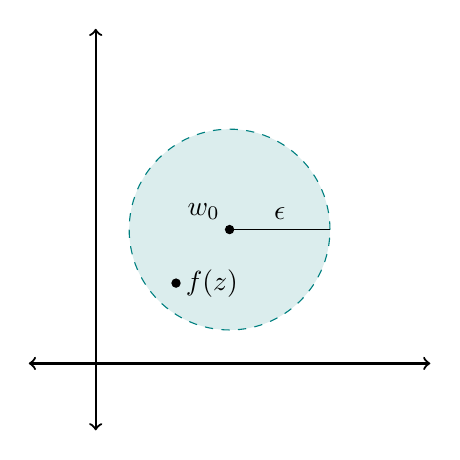
\begin{tikzpicture}[scale=0.85]
    \draw[<->,thick] (-1,0)--(5,0);
	\draw[<->,thick] (0,-1)--(0,5);
	\filldraw[teal,fill opacity=1/7,dashed](2,2) circle (1.5);
    \draw[](2,2)--(3.5,2) node[sloped,midway,above]{$\epsilon$};
    \fill (2,2) circle (2pt) node[above left]{$w_0$};
    \fill (1.2,1.2) circle (2pt) node[right]{$f(z)$};
  \end{tikzpicture}\]
In this case we write $\lim_{z \to z_0}f(z) = w_0$ or $f(z) \to w_0,\ \text{as } z \to z_0$.\\
\\
Intuitively, the limit of $f$ at $z_0$ is $w_0$ if \[\text{"$f$ is arbitrarily close to $w_0$ eventually, that is sufficiently, near $z_0$".}\] How close? Within an error of $\epsilon$. How near, eventually? Within a distance of $\delta$.
\end{definition}

\medskip

\begin{example}
\lecmargin{10}
Let's show that $\lim_{z \to i} z^2 = -1$ using the definition.
\end{example}
\begin{proof}
Let $\epsilon > 0$ be arbitrary. Note that $\abs{z^2 - (-1)} = \abs{z - i}\abs{z + i}$. We make an initial estimate, suppose $0 < \abs{z - i} < 1$, then
\begin{align*}
\abs{z + i} &= \abs{z - i + 2i}\\[0.5em]
&\leq \abs{z - i} + \abs{2i}\\[0.5em]
&< 1 + 2\\[0.5em]
&= 3
\end{align*}
Now, if we choose $\delta = \min\set{\dfrac{\epsilon}{3},1}$, then if $0 < \abs{z - i} < \delta$ we get
\[0 < \abs{z - i} < 1\ \text{and}\ \frac{\epsilon}{3}\]
So,
\begin{align*}
\abs{z^2 - (-1)} &= \abs{z - i}\abs{z + i}\\[0.5em]
&< 3\abs{z - i},\quad \text{since $\abs{z - i} < 1$}\\[0.5em]
&< 3\cdot\frac{\epsilon}{3},\quad \text{since $\abs{z - i} < \frac{\epsilon}{3}$}\\[0.5em]
&= \epsilon
\end{align*}
Therefore $\lim_{z \to i} z^2 = -1$.
\end{proof}

\medskip

\begin{theorem}\label{limunique}
If $f$ has a limit at $z_0$, then it is unique.
\end{theorem}
\begin{proof}
Assume
\[\lim_{z \to z_0}f(z) = \alpha \quad \text{and} \quad \lim_{z \to z_0}f(z) = \beta\]
Consider an arbitrary $\epsilon > 0$, then we can find a $\delta_1 > 0$ such that
\[\text{if }\ 0 < \abs{z - z_0} < \delta,\quad \text{then }\ \abs{f(z) - \alpha}<\frac{\epsilon}{2}\]
and $\delta_2 > 0$ such that
\[\text{if }\ 0 < \abs{z - z_0} < \delta,\quad \text{then }\ \abs{f(z) - \beta}<\frac{\epsilon}{2}\]
Define $\delta \coloneqq \min\set{\delta_1,\delta_2} \leq \delta_1,\,\delta_2$, then if $0< \abs{z - z_0} < \delta$ we have
\begin{align*}
\abs{\alpha - \beta} &= \abs{f(z) - f(z) + \alpha - \beta}\\[0.5em]
&\leq \abs{\alpha - f(z)} + \abs{f(z) - \beta}\\[0.5em]
&= \abs{f(z) - \alpha} + \abs{f(z) - \beta}\\[0.5em]
&< \frac{\epsilon}{2} + \frac{\epsilon}{2}\\[0.5em]
&= \epsilon
\end{align*}
We have proven that $\abs{\alpha - \beta} < \epsilon$ for any $\epsilon > 0$. Now, suppose $\alpha \neq \beta$, then for $\epsilon = \abs{\alpha - \beta} > 0$ we get $\abs{\alpha - \beta} < \abs{\alpha - \beta}$, which is preposterous. Hence $\alpha = \beta$, and thus the limit is unique.
\end{proof}

\medskip

\begin{remark}
The reason we require that $z_0$ be an accumulation point of the domain of $f$ is just that we need to be sure that there are points $z$ of the domain that are arbitrarily close to $z_0$. That is, there are indeed points satisfying $0< \abs{z-z_0} < \delta$.\\[0.5em]
Our definition (i.e., the part that says $0 < \abs{z - z_0}$) does not require $z_0$ to be in the domain of $f$, and if $z_0$ is in the domain of $f$, the definition explicitly ignores the value of $f(z_0)$.
\end{remark}

\medskip

Uniqueness of limits can be used to show that a limit does not exist.
\begin{example}\label{limnotex}
The function $f(z) = \dfrac{\overline{z}}{z}$ has no limit at $0$.
\end{example}
\begin{proof}[Discussion of Example \ref{limnotex}]
Let $z = x + iy$, then
\[f(z) = \frac{x - iy}{x + iy}\]
Along the real axis, $\Im z = 0$, and so $z = x$, giving us $f(z) = \dfrac{x}{x} = 1$.\\[0.5em]
Along the imaginary axis, $\Re z = 0$, and so $z = y$, giving us $f(z) = \dfrac{-y}{y} = -1$.\\[0.5em]
Taking the limit along these axes gives us different values of the limit, $1$ and $-1$. Hence, by the uniqueness of limits, the limit doesn't exist.
\end{proof}

\bigskip

\subsection{Theorems on Limits}
%\begin{mdframed}
%\begin{center}
%{\Large Theorems on Limits}
%\end{center}
%\end{mdframed}

\begin{theorem}[Limit in terms of Real and Imaginary parts of a Function]\label{cmplxlimripart}
Suppose that
\[f(z) = f(x + iy) = u(x,y) + i\,v(x,y)\]
Then 
\[\lim_{x + iy \to x_0 + iy_0}f(x + iy) = u_0 + iv_0\]
if and only if
\[\lim_{(x,y) \to (x_0,y_0)}u(x,y) = u_0 \quad \text{and} \quad \lim_{(x,y) \to (x_0,y_0)}v(x,y) = v_0\]
\end{theorem}
\begin{proof}
$(\Rightarrow)$ Consider an arbitrary $\epsilon > 0$, then there exists a $\delta > 0$ such that if
\[0 < \abs{(x+iy) - (x_0 + iy_0)} < \delta\]
\[\text{then }\ \abs{f(x+iy) - (u_0 + iv_0)} = \abs{(u(x,y) + i\,v(x,y)) - (u_0 + iv_0)} < \epsilon\]
We first note that, by definition
\begin{align*}
\norm{(x,y) - (x_0,y_0)} &= \abs{(x+iy) - (x_0 + iy_0)}
\end{align*}
and the end of Discussion \ref{cmplxnorm} tells us that
\begin{align*}
\abs{u(x,y) - u_0} &\leq \abs{(u(x,y) + i\,v(x,y)) - (u_0 + iv_0)} < \epsilon\\[0.5em]
\abs{v(x,y) - v_0} &\leq \abs{(u(x,y) + i\,v(x,y)) - (u_0 + iv_0)} < \epsilon
\end{align*}
That is, we have that
\[\text{if }\ 0 < \norm{(x,y) - (x_0,y_0)} < \delta,\quad \text{then }\ \abs{u(x,y) - u_0} < \epsilon\ \ \text{and}\ \ \abs{v(x,y) - v_0} < \epsilon\]
Therefore,
\[\lim_{(x,y) \to (x_0,y_0)}u(x,y) = u_0 \quad \text{and} \quad \lim_{(x,y) \to (x_0,y_0)}v(x,y) = v_0\]\\[1em]
$(\Leftarrow)$ Consider an arbitrary $\epsilon > 0$, then there exists a $\delta_1 > 0$ such that
\[\text{if }\ 0 < \norm{(x,y) - (x_0,y_0)} < \delta_1,\quad \text{then }\ \abs{u(x,y) - u_0} < \frac{\epsilon}{2}\]
and there exists a $\delta_2 > 0$ such that
\[\text{if }\ 0 < \norm{(x,y) - (x_0,y_0)} < \delta_2,\quad \text{then }\ \abs{v(x,y) - v_0} < \frac{\epsilon}{2}\]
Define $\delta \coloneqq \min\set{\delta_1,\delta_2} \leq \delta_1,\,\delta_2$. Now, if
\[0 < \abs{(x+iy) - (x_0 + iy_0)} = \norm{(x,y) - (x_0,y_0)} < \delta\]
then
\begin{align*}
\abs{f(x+iy) - (u_0 + iv_0)} &= \abs{(u(x,y) + i\,v(x,y)) - (u_0 + iv_0)}\\[0.5em]
&= \abs{(u(x,y) - u_0) + i(v(x,y)- v_0)}\\[0.5em]
&\leq \abs{(u(x,y) - u_0)} + \abs{i(v(x,y)- v_0)},\ \text{by triangle identity}\\[0.5em]
&= \abs{(u(x,y) - u_0)} + \abs{i}\abs{(v(x,y)- v_0)}\\[0.5em]
&= \abs{(u(x,y) - u_0)} + \abs{(v(x,y)- v_0)}\\[0.5em]
&< \frac{\epsilon}{2} + \frac{\epsilon}{2}\\[0.5em]
&= \epsilon
\end{align*}
Therefore,
\[\lim_{x + iy \to x_0 + iy_0}f(x + iy) = u_0 + iv_0\]
\end{proof}

\medskip

\begin{theorem}[Limit Laws]\label{limlaw}
Suppose
\[\lim_{z \to z_0} f(z) = \alpha \quad \text{and} \quad \lim_{z \to z_0} g(z) = \beta\]
Then
\begin{itemize}
\item[(1)] $\lim_{z \to z_0} (f(z) + g(z)) = \alpha + \beta$
\item[(2)] $\lim_{z \to z_0} (f(z)\,g(z)) = \alpha\beta$
\item[(3)] $\lim_{z \to z_0} \dfrac{f(z)}{g(z)} = \dfrac{\alpha}{\beta}$, provided $\beta \neq 0$.
\end{itemize}
\end{theorem}
\begin{proof}
The proof follows from Theorem \ref{cmplxlimripart} and limit laws from Calculus.
\end{proof}

\medskip

\begin{example}\label{polycts}
Let $p(z)$ be a polynomial, then
\[\lim_{z \to z_0}p(z) = p(z_0)\]
Write $p(z) = a_0 + a_1z + \cdots + a_nz^n$, then by Theorem \ref{limlaw} we have
\begin{align*}
\lim_{z \to z_0}p(z) &= \lim_{z \to z_0}(a_0 + a_1z + \cdots + a_nz^n)\\[0.5em]
&= \lim_{z \to z_0} a_0 + \lim_{z \to z_0} a_1z + \cdots + \lim_{z \to z_0} a_nz^n,\ \text{by Theorem \ref{limlaw} (1)}\\[0.5em]
&= \lim_{z \to z_0} a_0 + \lim_{z \to z_0} a_1 \cdot \lim_{z \to z_0} z + \cdots + \lim_{z \to z_0} a_n \cdot \lim_{z \to z_0} z^n,\ \text{by Theorem \ref{limlaw} (2)}\\[0.5em]
&= a_0 + a_1z_0 + \cdots + a_nz_0^n,\ \text{by Theorem \ref{limlaw} (2) and }\lim_{z \to z_0} z = z_0\\[0.5em]
&= p(z_0)
\end{align*}\\[-2em]
\qed
\end{example}

\bigskip

\begin{definition}[Extended Complex Plane or the Riemann Sphere]
\lecmargin{11}
The \cdef{Extended\ Complex\ Plane} is the set $\cc$ together with a symbol $\infty$ called the \emph{point at infinity}, denoted $\widehat{\cc}$ or $\cc_\infty$.\\[0.5em]
There is a bijection between the extended complex plane and the unit sphere given by the \emph{stereographic projection}, and therefore the extended complex plane is also called the \cdef{Riemann\ Sphere}.\\
\[\begin{tikzpicture}
  \draw[dashed] (-6,-1.5) -- (4.5, -1.5) -- (6, 1.5) -- (-3.5,1.5) -- (-6,-1.5);
  \draw (0,0) circle (3);
  \draw[dashed] (0,0) ellipse (3 and 1);
  \draw[] (0,3) -- (4.5, -1);
  \fill[forest] (0,3) circle (2pt) node[above,yshift=2pt]{{\color{forest}$N$}};
  \fill (0, 0) circle (2pt);
  \fill (4.5, -1) circle (2pt) node[below left]{$z$};
  \fill (0.56, 2.502) circle (2pt) node[right,yshift=3pt,xshift=2pt]{\small$p$};
  \shade[fill=forest,fill opacity=1/8] (5,1.5) arc (0:-60:3.45) -- (4.5,-1.5) -- (6,1.5) -- (5,1.5);
  \draw[dashed] (5,1.5) arc (0:-60:3.45);
  \shade[fill=forest,fill opacity=1/8] (-4.75,-1.5) arc (0:-75:-3.1) -- (-3.5,1.5) -- (-6,-1.5) -- (-4.75,-1.5);
  \draw[dashed] (-4.75,-1.5) arc (0:-75:-3.1);
  \shade[fill=forest,fill opacity=1/8] (2,2.236) arc (113.5:66.5:-5) arc (-48.35:-131.8:-3);
  \draw[dashed] (2,2.236) arc (113.5:66.5:-5);
  \node[] at (4,2) {\Large$\cc$};
\end{tikzpicture}\]\\
The point $N$ (the north pole) corresponds to $\infty$, and any point $p$ on the sphere corresponds uniquely to a point $z \in \cc$ which is the unique point of intersection of the complex plane with the line passing through $N$ and $p$.
\end{definition}

\medskip

\begin{definition}[Neighbourhood of Infinity]
Let $\epsilon > 0$, the set
\[\setp{z\in \cc}{\abs{z} > \frac{1}{\epsilon}}\]
is called a \emph{neighbourhood of $\infty$}. Geometrically, a neighbourhood at infinity is the exterior of a circle centered at the origin, which corresponds to a neighbourhood of $N$ on the unit sphere.
\end{definition}

\medskip

\begin{discussion}
We can now easily give meaning to limits
\[\lim_{z \to z_0}f(z) = w_0\]
where $z_0$ and $w_0$ are allowed to be $\infty$. We replace the appropriate neighbourhood in  Definition \ref{limdef} with neighbourhoods of $\infty$.
\end{discussion}

\medskip

\begin{theorem}[Limits involving Infinity]\hfill
\begin{itemize}
\item[(1)] $\displaystyle\lim_{z \to z_0} \dfrac{1}{f(z)} = 0$ if and only if $\displaystyle\lim_{z \to z_0}f(z) = \infty$.
\item[(2)] $\displaystyle\lim_{z \to \infty}f(z) = \lim_{z \to 0} f\left(\dfrac{1}{z}\right)$, provided the limit exist.
\end{itemize}
\emph{Combining (1) and (2), we get \[\displaystyle\lim_{z \to 0} \dfrac{1}{f\left(\frac{1}{z}\right)} = 0\quad \text{if and only if} \quad \displaystyle\lim_{z \to \infty}f(z) = \infty.\]}
Bottom line, we can simplify limits involving $\infty$ to limits involving $0$.
\end{theorem}
\begin{proof}
The proofs are based on the simple observation that
\[\frac{1}{a} < b \quad \text{if and only if} \quad \frac{1}{b} < a\]
for non-zero real numbers $a$ and $b$.
\begin{itemize}
\item[(1)] Now $\displaystyle\lim_{z \to z_0} \dfrac{1}{f(z)} = 0$ if and only if for every $\epsilon > 0$ there exists $\delta > 0$ such that 
\[\text{if }\ 0 < \abs{z - z_0} < \delta,\quad \text{then }\ \frac{1}{\abs{f(z)}} = \abs{\frac{1}{f(z)} - 0}< \epsilon\]
if and only if for every $\epsilon > 0$ there exists $\delta > 0$ such that 
\[\text{if }\ 0 < \abs{z - z_0} < \delta,\quad \text{then }\ \abs{f(z)}>\frac{1}{\epsilon}\]
if and only if
$\displaystyle\lim_{z \to z_0}f(z) = \infty$.
\item[(2)] $\displaystyle\lim_{z \to \infty}f(z) = \alpha$ if and only if for every $\epsilon > 0$ there exists $\delta > 0$ such that 
\[\text{if }\ \abs{z} > \frac{1}{\delta},\quad \text{then }\ \abs{f(z) - \alpha}< \epsilon\]
if and only if for every $\epsilon > 0$ there exists $\delta > 0$ such that 
\[\text{if }\ 0 < \abs{\frac{1}{z}} < \delta,\quad \text{then }\ \abs{f(z) - \alpha} < \epsilon\]
if and only if, by replacing $z$ with $1/z$, $\displaystyle\lim_{z \to 0}\,f\left(\dfrac{1}{z}\right) = \alpha$.
\end{itemize}
\end{proof}

\medskip

\begin{example}
We want to show $\displaystyle \lim_{z \to \infty} \frac{2z^4 + 1}{z^3 + 1} = \infty$. This is equivalent to showing
\[\lim_{z \to 0} \frac{1}{f(1/z)} = \lim_{z \to 0} \frac{(1/z)^3 + 1}{2(1/z)^4 + 1} = 0,\quad \text{for }f(z) = \frac{2z^4 + 1}{z^3 + 1}\]
Note that,
\begin{align*}
\lim_{z \to 0} \frac{(1/z)^3 + 1}{2(1/z)^4 + 1}&= \lim_{z \to 0} \frac{\frac{1 + z^3}{z^3}}{\frac{2 + z^4}{z^4}}\\[0.5em]
&= \lim_{z \to 0}\ z\cdot\frac{1 + z^3}{2 + z^4}\\[0.5em]
&= 0\cdot\frac{1}{2}\\[0.5em]
&= 0
\end{align*}
Therefore $\displaystyle \lim_{z \to \infty} \frac{2z^4 + 1}{z^3 + 1} = \infty$.
\end{example}

\medskip

\begin{example}[in-class]
Show $\displaystyle \lim_{z \to \infty} \frac{2 + z^5}{z^2 + 3} = \infty$.
\end{example}
\begin{proof}[Answer]
This is equivalent to showing
\[\lim_{z \to 0} \frac{1}{f(1/z)} = \lim_{z \to 0} \frac{(1/z)^2 + 3}{2 + (1/z)^5} = 0,\quad \text{for }f(z) = \frac{2 + z^5}{z^2 + 3}\]
Note that,
\begin{align*}
\lim_{z \to 0} \frac{(1/z)^2 + 3}{2 + (1/z)^5} &= \lim_{z \to 0} \frac{\frac{1 + 3z^2}{z^2}}{\frac{2z^5 + 1}{z^5}}\\[0.5em]
&= \lim_{z \to 0}\ z^3\cdot\frac{1 + 3z^2}{2z^5 + 1}\\[0.5em]
&= 0^3\cdot\frac{1}{1}\\[0.5em]
&= 0
\end{align*}
Therefore $\displaystyle \lim_{z \to \infty} \frac{2 + z^5}{z^2 + 3} = \infty$.
\end{proof}

\bigskip

\subsection{Continuous Functions}
%\begin{mdframed}
%\begin{center}
%{\Large Continuous Functions}
%\end{center}
%\end{mdframed}

\begin{definition}[Continuous Functions]
A function $f: G \to \cc$ is \emph{continuous at $z_0 \in G$} if either $z_0$ is an isolated point or 
\[\lim_{z \to z_0}\,f(z) = f(z_0) = f\left(\lim_{z\to z_0}\,z\right)\]
That is, for all $\epsilon > 0$, there exists a $\delta > 0$ such that
\[\text{if }\ 0 < \abs{z - z_0} < \delta,\quad \text{then }\ \abs{f(z) - f(z_0)}<\epsilon.\]
A function is \cdef{continuous} if it is continuous at every point in its domain.\\
\\
By the limit laws (Theorem \ref{limlaw}), sum, product and quotient of continuous functions are continuous (whenever and wherever defined).
\end{definition}

\medskip

\begin{theorem}[Composition of Continuous Functions]\label{composcont}
Suppose we have two functions $f:G_1 \to \cc$ and $g: G_2 \to \cc$ such that $f(G_1) \subseteq G_2$. If $f$ is continuous at $z_0$ and $g$ is continuous at $f(z_0)$, then $g\circ f$ is continuous at $z_0$. That is,
\[\lim_{z \to z_0}g(f(z)) = g(f(z_0)) = g\left(\lim_{z\to z_0}f(z)\right) = g\left(f\left(\lim_{z\to z_0}\,z\right)\right)\]
Therefore, if $f$ and $g$ are continuous, so is $g\circ f$.
\end{theorem}
\begin{proof}
By continuity of $g$ at $f(z_0)$, for an arbitrary $\epsilon > 0$, there exists a $\delta_1 > 0$ such that
\[\text{if }\ 0 < \abs{w - f(z_0)} < \delta_1,\quad \text{then }\ \abs{g(w) - g(f(z_0))}<\epsilon.\]
Now, by continuity of $f$ at $z_0$, for $\delta_1 > 0$, there exists a $\delta > 0$ such that
\[\text{if }\ 0 < \abs{z - z_0} < \delta,\quad \text{then }\ \abs{f(z) - f(z_0)}<\delta_1.\]
With these two statements, we have that 
\[\text{if }\ 0 < \abs{z - z_0} < \delta,\quad \text{then }\ \abs{g(f(z)) - g(f(z_0))}<\epsilon.\]
Therefore $g\circ f$ is continuous at $z_0$.
\end{proof}

\medskip

\begin{theorem}
\lecmargin{12}
Suppose $f: G \to \cc$ is continuous at $z_0$ and $f(z_0) \neq 0$, then there exists a $\delta > 0$ such that $f(z) \neq 0$ for all $z \in D_\delta(z_0)$. That is, $\abs{f(z)} > 0$ for all $z \in D_\delta(z_0)$.
\end{theorem}
\begin{proof}
Since $f$ is continuous and non-zero at $z_0$, for $\epsilon = \dfrac{\abs{f(z_0)}}{2} > 0$ there exists a $\delta > 0$ such that
\[\text{if }\ z \in D_\delta(z_0),\quad \text{then }\ \abs{f(z) - f(z_0)}< \frac{\abs{f(z_0)}}{2}.\]
For such a $z$, the reverse triangle inequality gives us
\[\abs{\abs{f(z)} - \abs{f(z_0)}} \leq \abs{f(z) - f(z_0)}< \frac{\abs{f(z_0)}}{2};\quad \text{so, }\ -\frac{\abs{f(z_0)}}{2} < \abs{f(z)} - \abs{f(z_0)} < \frac{\abs{f(z_0)}}{2}\]
since the former is the absolute value of real numbers. Therefore, adding $\abs{f(z_0)}$ to this inequality gives us
\[\abs{f(z)} > \frac{\abs{f(z_0)}}{2} > 0\]
as needed.
\end{proof}

\medskip

\begin{theorem}[Continuity in terms of Real and Imaginary parts of a Function]\label{contpart}
Suppose that 
\[f(z) = f(x + iy) = u(x,y) + i\,v(x,y).\]
Then $f$ is continuous at $z_0 = x_0 + iy_0$ if and only if $u$ and $v$ are continuous at $(x_0,y_0)$.
\end{theorem}
\begin{proof}
This is directly follows from Theorem \ref{cmplxlimripart}.
\end{proof}

\medskip

\begin{definition}[Compact Sets]
A subset of $\cc$ is said to be \cdef{compact} if it is closed and bounded.
\end{definition}

\medskip

\begin{definition}[Bounded Functions]
A function $f: G \to \cc$ is said to be a \cdef{bounded\ function} if the image $f(G)$ is bounded. Equivalently, if there exists $M > 0$ such that $\abs{f(z)} \leq M$ for every $z \in G$.
\end{definition}

\medskip

\begin{theorem}[Extreme Value Theorem]\label{evt}
Suppose $K \subseteq \cc$ is compact, and $f: K \to \cc$ is continuous. Then $f$ is bounded, that is there exists an $M > 0$ such that $\abs{f(z)} \leq M$ for all $z \in K$, and there exists a $z_0 \in K$ such that $\abs{f(z_0)} = M$.
\end{theorem}
\begin{proof}
Since $f = u + iv$ is continuous, so are $u,v:\rr^2 \to \rr$ by Theorem \ref{contpart}.  Hence, so is
\[\abs{f(z)} = \abs{f(x + iy)} = \sqrt{u(x,y)^2 + v(x,y)^2}\]
as it's obtained as a sum, product and composition of continuous functions. This result then follows from standard Calculus, since $\abs{f}$ is a real-valued function.
\end{proof}

\bigskip

\subsection{Complex-Differentiable Functions}
%\begin{mdframed}
%\begin{center}
%{\Large Complex-Differentiable Functions}
%\end{center}
%\end{mdframed}

\begin{definition}[Derivative]\label{cmplxder}
Consider a function $f:G \to \cc$, the \cdef{derivative} \emph{of $f$ at $z_0 \in G$} is the limit
\[\frac{d}{dz}(f(z_0)) = f'(z_0) \coloneqq \lim_{z \to z_0}\frac{f(z) - f(z_0)}{z - z_0}\]
If the limit exists, we say $f$ is \emph{differentiable at $z_0$}.\\[0.5em]
A function is \cdef{differentiable} if it is differentiable at every point in its domain.
\end{definition}
Letting $h = \Delta_{z_0}z = z - z_0$, the limit can also be written as
\[f'(z_0) = \lim_{h \to 0}\frac{f(z_0 + h) - f(z_0)}{h}\]

\medskip

\begin{example}
Consider $f(z) = z^2$, then
\begin{align*}
f'(z) = \lim_{h \to 0}\frac{f(z + h) - f(z)}{h} &= \lim_{h \to 0}\frac{(z + h)^2 - z^2}{h}\\[0.5em]
&= \lim_{h \to 0}\frac{2zh + h^2}{h}\\[0.5em]
&= \lim_{h \to 0}\,2z + h\\[0.5em]
&= 2z
\end{align*}
\end{example}

\medskip

\begin{example}\label{normdiffexistence}
\lecmargin{13}
Where is $f(z) = \abs{z}^2$ differentiable?\\[1em]
Consider $z \in \cc$ and an arbitrary $h \in \cc$, then we compute
\begin{align*}
f(z + h) - f(z) &= \abs{z + h}^2 - \abs{z}^2\\[0.5em]
&= (z + h)\overline{(z + h)} - z\overline{z}\\[0.5em]
&= z\overline{z} + z\overline{h} + \overline{z}h + h\overline{h} - z\overline{z}\\[0.5em]
&= z\overline{h} + \overline{z}h + h\overline{h}
\end{align*}
Then 
\[\frac{f(z + h) - f(z)}{h} = \frac{z\overline{h} + \overline{z}h + h\overline{h}}{h} = z\,\frac{\overline{h}}{h} + \overline{z} + \overline{h}\]
Along the real axis, $h = \overline{h}$, we have
\[\frac{f(z + h) - f(z)}{h} = z + \overline{z} + h;\]
therefore, as $h \to 0$, the limit is $z + \overline{z}$. Along the imaginary axis, $h = -\overline{h}$, we have
\[\frac{f(z + h) - f(z)}{h} = -z + \overline{z} - h;\]
therefore, as $h \to 0$, the limit is $-z + \overline{z}$.\\
\\
Since limits are unique, if $f'(z)$ exists, then $z + \overline{z} = -z + \overline{z}$, which gives us $z = 0$. That is, if $f'(z)$ exists, it only exists for $z = 0$. So, does $f'(0)$ exist?
\[f'(0) = \lim_{h \to 0}\frac{f(h) - f(0)}{h} = \lim_{h \to 0}\frac{h\overline{h}}{h} = \lim_{h \to 0}\overline{h} = 0\]
\end{example}

\medskip

\begin{proposition}[Differentiable Functions are Continuous]
If $f$ is differentiable at $z_0$, then $f$ is continuous at $z_0$.
\end{proposition}
\begin{proof}
Suppose $f$ is differentiable at $z_0$, then
\[\lim_{z \to z_0}f(z) - f(z_0) = \left(\lim_{z \to z_0}\frac{f(z) - f(z_0)}{z - z_0}\right)\left(\lim_{z \to z_0}\,z - z_0\right) = f'(z_0)\cdot 0 = 0\]
Therefore $\lim_{z \to z_0}f(z) = f(z_0)$, and hence $f$ is continuous at $z_0$.
\end{proof}

\medskip

\begin{theorem}[Differentiation Laws]
Suppose $f$ and $g$ are differentiable at $z$. Then,
\begin{itemize}[itemsep=1em]
\item[(1)] $(c)' = 0$, for every $c \in \cc$.
\item[(2)] $(c\cdot f)'(z) = c\cdot f'(z)$, for every $c \in \cc$.\hfill \emph{(Constant Rule)}
\item[(3)] $(z^n)' = nz^{n-1}$, for every $n \in \zz$ (assume $z \neq 0$ for $n<0$).\hfill \emph{(Power Rule)}
\item[(4)] $(f + g)'(z) = f'(z) + g'(z)$.\hfill \emph{(Sum Rule)}
\item[(5)] $(fg)'(z) = f'(z)g(z) + f(z)g'(z)$.\hfill \emph{(Product Rule)}
\item[(6)] $\left(\dfrac{f}{g}\right)'(z) = \dfrac{f'(z)g(z) - f(z)g'(z)}{g(z)^2}$, provided $g(z) \neq 0$ \hfill \emph{(Quotient Rule)}
\end{itemize}
\end{theorem}
\begin{proof}
(1) and (4) are proved directly using the limit definition, (2) can be proved directly or using (1) and (5), while (3) can be proven inductively using (5) for positive $n$ and (6) for negative $n$. 
\begin{itemize}
\item[(5)] We first compute
\begin{align*}
f(z + h)g(z + h) - f(z)g(z) &= f(z + h)g(z + h) - f(z)g(z) + f(z + h)g(z) - f(z + h)g(z)\\[0.5em]
&= f(z + h)(g(z + h) - g(z)) + g(z)(f(z + h) - f(z))
\end{align*}
So,
\begin{align*}
(fg)'(z) &= \lim_{h \to 0}\frac{f(z + h)g(z + h) - f(z)g(z)}{h}\\[0.5em]
&= \lim_{h \to 0}\frac{f(z + h)(g(z + h) - g(z))}{h} + \lim_{h \to 0}\frac{g(z)(f(z + h) - f(z))}{h}\\[0.5em]
&= \lim_{h \to 0}f(z + h)\cdot\lim_{h \to 0}\frac{g(z + h) - g(z)}{h} + g(z)\lim_{h \to 0}\frac{f(z + h) - f(z)}{h}\\[0.5em]
&= f(z)g'(z) + g(z)f'(z)
\end{align*}
\item[(6)] We first compute
\begin{align*}
\frac{1}{g(z + h)} - \frac{1}{g(z)} &= \frac{g(z) - g(z + h)}{g(z)g(z + h)}\\[0.5em]
&= -\frac{g(z+h) - g(z)}{g(z)g(z + h)}
\end{align*}
So,
\begin{align*}
\left(\dfrac{1}{g}\right)'(z) &= \lim_{h \to 0}\frac{\dfrac{1}{g(z + h)} - \dfrac{1}{g(z)}}{h}\\[0.5em]
&= \lim_{h \to 0}-\frac{g(z+h) - g(z)}{g(z)g(z + h)}\cdot\frac{1}{h}\\[0.5em]
&= -\lim_{h \to 0}\frac{g(z+h) - g(z)}{h}\cdot\lim_{h \to 0}\frac{1}{g(z)g(z + h)}\\[0.5em]
&= -\frac{g'(z)}{g(z)^2}
\end{align*}
(6) then follows from the computation above and using (5) on $\dfrac{f(z)}{g(z)} = f(z)\cdot\dfrac{1}{g(z)}$.
\end{itemize}
\vspace*{-\baselineskip}
\end{proof}

\medskip

\begin{proposition}[Chain Rule]
Suppose we have two functions $f:G_1 \to \cc$ and $g: G_2 \to \cc$ such that $f(G_1) \subseteq G_2$. If $f$ is differentiable at $z_0$ and $g$ is differentiable at $f(z_0)$, then $g\circ f$ is differentiable at $z_0$ and
\[(g\circ f)'(z_0) = g'(f(z_0))\cdot f'(z_0)\]
\end{proposition}
\begin{proof}
Let's start by defining an auxiliary function on $G_2$
\[\phi(w) = \begin{cases} \dfrac{g(w) - g(f(z_0))}{w - f(z_0)} - g'(f(z_0)) & w \neq f(z_0)\\[0.5em] 0 & w = f(z_0) \end{cases}\]
Since $g$ is differentiable at $f(z_0)$, then $\lim_{w \to f(z_0)}\phi(w) = 0 = \phi(f(z_0))$ and therefore $\phi$ is continuous at $f(z_0)$. Furthermore, since $f$ is differentiable at $z_0$, it is continuous at $z_0$. So $\lim_{z \to z_0}\phi(f(z)) = \phi(f(z_0)) = 0$ by Theorem \ref{composcont}.\\[1em]
Rewriting the above expression, we get the following expression which is valid on all of $G_2$.
\[g(w) - g(f(z_0)) = (w - f(z_0))(\phi(w) + g'(f(z_0)))\]
Now, for $w = f(z) \in f(G_1)$, we have
\begin{align*}
\frac{g(f(z)) - g(f(z_0))}{z - z_0} &= \frac{(f(z) - f(z_0))(\phi(f(z)) + g'(f(z_0)))}{z - z_0}\\[0.5em]
&= (\phi(f(z)) + g'(f(z_0)))\cdot\frac{f(z) - f(z_0)}{z - z_0}
\end{align*}
Therefore, 
\begin{align*}
(g\circ f)'(z_0) &= \lim_{z \to z_0}\frac{g(f(z)) - g(f(z_0))}{z - z_0}\\[0.5em]
&= \lim_{z \to z_0}(\phi(f(z)) + g'(f(z_0)))\cdot\lim_{z \to z_0}\frac{f(z) - f(z_0)}{z - z_0}\\[1em]
&= g'(f(z_0))\cdot f'(z_0),\ \text{since $\lim_{z \to z_0}\phi(f(z)) = 0$}
\end{align*}
\end{proof}

\bigskip

\subsection{Cauchy-Riemann Equations}
%\begin{mdframed}
%\begin{center}
%{\Large Cauchy-Riemann Equations}
%\end{center}
%\end{mdframed}
%
%When considering a real-valued function $f : \rr^2 \to \rr$ of two variables, there is no notion of the derivative of a function. For such a function, we instead only have partial derivatives $f_x(x_0,y_0)$ and $f_y(x_0,y_0)$ (and also directional derivatives) which depend on the way in which we approach a point $(x_0, y_0) \in \rr^2$. For a complex-valued function $f(z)$, we now have a new concept of the derivative $f'(z_0)$, which by definition cannot depend on the way in which we approach a point $z_0 \in \cc$. It is then natural expect a relationship between the complex derivative $f'(z_0)$ and the partial derivatives of $\Re f$ and $\Im f$, which are real-values functions. 
%
\medskip
%
\begin{theorem}[Cauchy-Riemann Equations]\label{crequations}
\lecmargin{14}
Suppose that 
\[f(z) = f(x + iy) = u(x,y) + i\,v(x,y)\]
is differentiable at $z_0 = x_0 + iy_0$. Then
\begin{itemize}
\item[(a)] the first order partial derivatives of $u$ and $v$ exist at $(x_0,y_0)$ and satisfy the \cdef{Cauchy\text{-}Riemann\ Equations}
\begin{align*}\label{creqex}
u_x(x_0,y_0) &= v_y(x_0,y_0)\\[-0.5em]
\tag{CR}\\[-0.5em]
u_y(x_0,y_0) &= -v_x(x_0,y_0)
\end{align*}
\item[(b)] $f'(z_0) = u_x(x_0,y_0) + i\,v_x(x_0,y_0) = v_y(x_0,y_0) - i\,u_y(x_0,y_0)$.
\end{itemize}
\end{theorem}
\begin{proof}
Since $f$ is differentiable at $z_0$, we have, where we let $h = s + it$
\begin{align*}
f'(z_0) &= \lim_{h\to 0}\frac{f(z_0 + h) - f(z_0)}{h}\\[0.5em]
&= \lim_{h\to 0}\frac{f((x_0 + s) + i(y_0 + t)) - f(x_0 + iy_0)}{h}\\[0.5em]
&= \lim_{h\to 0}\frac{u(x_0 + s,y_0 + t) - u(x_0,y_0)}{h} + i\cdot\lim_{h\to 0}\frac{v(x_0 + s,y_0 + t) - v(x_0,y_0)}{h}
\end{align*}
As we know by now, we must get the same result if we restrict $h$ to be on the real axis and if we restrict it to be on the imaginary axis. In the former case, $t = 0$, giving us
\begin{align*}
f'(z_0) &= \lim_{s\to 0}\frac{u(x_0 + s,y_0) - u(x_0,y_0)}{s} + i\cdot\lim_{s\to 0}\frac{v(x_0 + s,y_0) - v(x_0,y_0)}{s}\\[0.5em]
&= u_x(x_0,y_0) + i\,v_x(x_0,y_0)
\end{align*}
In the latter case, $s = 0$, giving us
\begin{align*}
f'(z_0) &= \lim_{t\to 0}\frac{u(x_0,y_0 + t) - u(x_0,y_0)}{it} + i\cdot\lim_{t\to 0}\frac{v(x_0,y_0 + t) - v(x_0,y_0)}{it}\\[0.5em]
&= \frac{1}{i}\cdot\lim_{t\to 0}\frac{u(x_0,y_0 + t) - u(x_0,y_0)}{t} + \lim_{t\to 0}\frac{v(x_0,y_0 + t) - v(x_0,y_0)}{t}\\[0.5em]
&= -i\,u_y(x_0,y_0) + v_y(x_0,y_0)
\end{align*}
Therefore
\[u_x(x_0,y_0) + i\,v_x(x_0,y_0) = f'(z_0) = v_y(x_0,y_0)-i\,u_y(x_0,y_0),\]
and hence $u_x(x_0,y_0) = v_y(x_0,y_0)$ and $u_y(x_0,y_0) = -v_x(x_0,y_0)$.
\end{proof}

\medskip

The Cauchy-Riemann equations (\ref{creqex}) are a \emph{necessary} condition for $f'$ to exist. We can use them to locate possible points where the derivative does not exist but not necessarily conclude where and if the derivative exists.
\begin{example}\label{necessarycr}\hfill
\begin{itemize}
\item[(1)] Consider $f(z) = \abs{z}^2 = x^2 + y^2$, so $u(x,y) = x^2 + y^2$ and $v(x,y) = 0$. The partial derivatives at $(x,y)$ are
\begin{align*}
u_x &= 2x & v_x &= 0\\[0.5em]
u_y &= 2y & v_y &= 0
\end{align*}
Therefore, the Cauchy-Riemann equations (\ref{creqex}) are only satisfied at $(x,y) = (0,0)$. Hence $f$ is not differentiable at any $z \neq 0$. Again, note that this does not say anything about the existence of $f'(0)$.
\item[(2)] Consider $f(z) = \overline{z} = x - iy$, so $u(x,y) = x$ and $v(x,y) = -y$. The partial derivatives at $(x,y)$ are
\begin{align*}
u_x &= 1 & v_x &= 0\\[0.5em]
u_y &= 0 & v_y &= -1
\end{align*}
Note that $u_x \neq v_y$ for all $(x,y)$ and therefore the Cauchy-Riemann equations (\ref{creqex}) are satisfied for no $(x,y)$. Hence $f$ is nowhere complex-differentiable.
\item[(3)] (in-class) Consider $f(z) = (z + i\overline{z})^2$, let's simplify $f$ to identify its real and imaginary parts $u(x,y)$ and $v(x,y)$.
\begin{align*}
f(z) &= (z + i\overline{z})^2\\[0.5em]
 &= z^2 - \overline{z}^2 + 2iz\overline{z}\\[0.5em]
 &= (z + \overline{z})(z - \overline{z}) + 2i\abs{z}^2\\[0.5em]
 &= (2\Re z)(2i \Im z) + 2i\abs{z}^2
 = 2i(\abs{z}^2 + \Re z \cdot \Im z)
\end{align*}
\begin{align*}
f(x + iy) &= 2i(x^2 + y^2 + 2xy)\\[0.5em]
&= 2i(x + y)^2
\end{align*}
Therefore $u(x,y) = 0$ and $v(x,y) = 2(x + y)^2$. The partial derivatives at $(x,y)$ are
\begin{align*}
u_x &= 0 & v_x &= 4(x + y)\\[0.5em]
u_y &= 0 & v_y &= 4(x + y)
\end{align*}
Therefore, the Cauchy-Riemann equations (\ref{creqex}) are satisfied if and only if $4(x + y) = 0$, if and only if $y = -x$. Hence $f$ is not differentiable any $z \in \cc$ such that $\Im z \neq -\Re z$.
\end{itemize}
\end{example}

\medskip

As commented, the Cauchy-Riemann equations (\ref{creqex}) are not a \emph{sufficient} condition for the existence of the derivative as the example below shows. Problem \ref{prob 7.1} gives another example.
\begin{example}\label{onlynecescr}
Consider
\[f(z) = \begin{cases}\dfrac{\overline{z}^2}{z} = \dfrac{\overline{z}^3}{\abs{z}^2} & z \neq 0\\[1em] 0 & z = 0 \end{cases}\]
Then,
\[u(x,y) = \begin{cases}\dfrac{x^3 - 3xy^2}{x^2 + y^2} & (x,y) \neq (0,0)\\[1em] 0 & (x,y) = (0,0) \end{cases} \qquad \text{and} \qquad v(x,y) = \begin{cases}\dfrac{y^3 - 3x^2y}{x^2 + y^2} & (x,y) \neq (0,0)\\[1em] 0 & (x,y) = (0,0) \end{cases}\]
We show that $u$ and $v$ satisfy the Cauchy-Riemann equations (\ref{creqex}) at $(0,0)$.
\begin{align*}
u_x(0,0) &= \lim_{s \to 0}\frac{u(s,0) - u(0,0)}{s} = \lim_{s \to 0}\frac{\dfrac{s^3}{s^2} - 0}{s} = 1\\[0.5em]
u_y(0,0) &= \lim_{t \to 0}\frac{u(0,t) - u(0,0)}{t} = \lim_{t \to 0}\frac{0 - 0}{t} = 0  \\[1em]
v_x(0,0) &= \lim_{s \to 0}\frac{v(s,0) - v(0,0)}{s} = \lim_{s \to 0}\frac{0 - 0}{s} = 0\\[0.5em]
v_y(0,0) &= \lim_{t \to 0}\frac{v(0,t) - v(0,0)}{t} = \lim_{t \to 0}\frac{\dfrac{t^3}{t^2} - 0}{t} = 1
\end{align*}
Therefore $u_x(0,0) = 1 = v_y(0,0)$ and $u_y(0,0) = 0 = -v_x(0,0)$, and hence the Cauchy-Riemann equations (\ref{creqex}) are satisfied. But $f'(0)$ does not exist, as seen in Problem \ref{prob 6.6}.
\end{example}

\medskip

Imposing certain existence and continuity conditions on the first order partial derivatives of $u$ and $v$, the Cauchy-Riemann equations (\ref{creqex}) can be upgraded to a sufficient condition for differentiability.
\begin{theorem}[Sufficient Conditions for Differentiability]\label{crsuff}
Consider a function \[f(z) = f(x + iy) = u(x,y) + i\,v(x,y)\]
and a $z_0$ in the domain of $f$, such that
\begin{itemize}
\item[(a)] the first order partial derivatives of $u$ and $v$ exist and are continuous in an open disk centered at $z_0$; and
\item[(a)] the Cauchy-Riemann equations (\ref{creqex}) are satisfied at $(x_0,y_0)$.
\end{itemize}
Then $f'(z_0)$ exists and is given by $u_x(x_0,y_0) + i\,v_x(x_0,y_0) = v_y(x_0,y_0)-i\,u_y(x_0,y_0)$.
\end{theorem}
\begin{proof}
We skip the proof. You can find a proof in \cite[Section~22, Page~66]{brown2009complex}.
\end{proof}

\medskip

\begin{example}
Let's revisit examples from Example \ref{necessarycr} and \ref{onlynecescr}.
\begin{itemize}
\item[(1)] Consider $f(z) = \abs{z}^2 = x^2 + y^2$, we noted that $u(x,y) = x^2 + y^2$ and $v(x,y) = 0$. We have seen that the only point where $f(z)$ can be differentiable is $z = 0$. The partial derivatives in a neighbourhood of $(0,0)$ are
\begin{align*}
u_x &= 2x & v_x &= 0\\[0.5em]
u_y &= 2y & v_y &= 0
\end{align*}
which clearly exist and are continuous. We have also seen that the Cauchy-Riemann equations (\ref{creqex}) are satisfied at $(0,0)$, trivially. Therefore $f'(0)$ exists and \[f'(0) = u_x(0,0) + i\,v_x(0,0) = 0.\]

\item[(2)] Consider $f(z) = (z + i\overline{z})^2$, we noted that $u(x,y) = 0$ and $v(x,y) = 2(x + y)^2$. We have seen that the only point where $f(z)$ can be differentiable are $z = x + iy \in \cc$ such that $y = \Im z = -\Re z = -x$. That is, at points of the form $(x,-x)$. The partial derivatives in a neighbourhood of $(x,-x)$ are
\begin{align*}
u_x &= 0 & v_x &= 4(x + y)\\[0.5em]
u_y &= 0 & v_y &= 4(x + y)
\end{align*}
which clearly exist and are continuous. Note the Cauchy-Riemann equations (\ref{creqex}) are satisfied at $(x,-x)$ trivially, since \[u_x(x,-x) = u_y(x,-x) = v_x(x,-x) = v_y(x,-x) = 0.\]
Therefore $f'(z)$ exists, for $z = x - ix$, and \[f'(z) = u_x(x,-x) + i\,v_x(x,-x) = 0.\]

\item[(3)] The reason Example \ref{onlynecescr} doesn't contradict Theorem \ref{crsuff} is because, $u_x$, in particular, is not continuous at $(0,0)$. Note that we have
\[u(x,y) = \begin{cases}\dfrac{x^3 - 3xy^2}{x^2 + y^2} & (x,y) \neq (0,0)\\[1em] 0 & (x,y) = (0,0) \end{cases}\]
For $(x,y) \neq (0,0)$, we compute $u_x(x,y)$ using the quotient rule, while we have already computed $u_x(0,0) = 1$ in Example \ref{onlynecescr}, giving us
\[u_x(x,y) = \begin{cases}\dfrac{x^4 + 6x^2y^2 - 3y^4}{(x^2 + y^2)^2} & (x,y) \neq (0,0)\\[1em] 1 & (x,y) = (0,0) \end{cases}\]
Suppose $u_x(x,y)$ is continuous at $(0,0)$, then we have
\[\lim_{(x,y) \to (0,0)}u_x(x,y) = \lim_{(x,y) \to (0,0)}\dfrac{x^4 + 6x^2y^2 - 3y^4}{(x^2 + y^2)^2} = u_x(0,0) = 1\]
Restricting the limit along the $y$-axis, where $x = 0$, we get
\[1 = \lim_{(0,y) \to (0,0)}\dfrac{-3y^4}{(y^2)^2} = \lim_{y \to 0}\dfrac{-3y^4}{y^4} = -3,\]
a contradiction. Hence, $u_x(x,y)$ is not continuous at $(0,0)$.
\end{itemize}
\end{example}

\medskip

\begin{example}[Complex Exponential]\label{expcmplxeg}
\lecmargin{15}
Define, for any $z = x + iy \in \cc$
\[\exp(z) = e^z \coloneqq e^xe^{iy} = e^x(\cos y + i\,\sin y)\]
the \emph{complex exponential function}. Note that $e^x$ is the usual real exponential and $e^{iy}$ is given by Euler's formula (Definition \ref{eulerform}). Here, 
\[u(x,y) = e^x\cos y \quad \text{and} \quad v(x,y) = e^x\sin y\]
We then see that
\begin{align*}
u_x &= e^x\cos y = v_y,\\[0.5em] v_x &= -e^x\sin y = -u_y;
\end{align*}
so $\exp$ satisfies the Cauchy-Riemann equations (\ref{creqex}) everywhere. Furthermore, $u_x,\,u_y,\,v_x$ and $v_y$ are everywhere defined and continuous. Hence $\exp$ is everywhere complex-differentiable, an \emph{entire} function. Furthermore $\exp(z)' = u_x + iv_x = e^x\cos y + ie^x\sin y = \exp(z)$.
\end{example}

\medskip

\begin{discussion}[Polar Cauchy-Riemann Equations]
Recall that if the domain of a function $f$ is contained in $\cc^*$ or restricted to within $\cc^*$, one can express in polar coordinates at $z = re^{i\theta}$ as
\[f(z) = f(re^{i\theta}) = u(r,\theta) + i\,v(r,\theta)\]
Then, the Cauchy-Riemann equations (\ref{creqex}) at a point $(r_0,\theta_0)$ can be expressed in polar coordinates, \cdef{Polar\ Cauchy\text{-}Riemann\ Equations} (see Problem \ref{prob 7.3})
\begin{align*}\label{pcreqex}
ru_r &= v_\theta\\[-0.5em]
\tag{Polar CR}\\[-0.5em]
u_\theta &= -rv_r
\end{align*}
and a differentiable function at $z_0 = r_0e^{i\theta_0}$ is then expressed as \[f'(z_0) = f'(r_0e^{i\theta_0}) = e^{-i\theta_0}(u_r(r_0,\theta_0) + i\,v_r(r_0,\theta_0)).\]
\end{discussion}

\medskip

\begin{example}
Consider the function
\[f(z) = f(re^{i\theta}) = \sqrt{r}\,e^{i\frac{\theta}{2}} ,\]
where $r > 0$ and $-\pi < \theta < \pi$. This is the function that outputs the principal square root of $z$. We compute $f'(z)$ at $z = re^{i\theta}$ using the polar form of Theorem \ref{crsuff}. We first note that
\[f(z) = \underbrace{\sqrt{r}\cos\left(\frac{\theta}{2}\right)}_{u(r,\theta)} + i\underbrace{\sqrt{r}\sin\left(\frac{\theta}{2}\right)}_{v(r,\theta)}\]
Now, we compute
\begin{align*}
ru_r &= r\frac{1}{2\sqrt{r}}\cos\left(\frac{\theta}{2}\right) = \frac{\sqrt{r}}{2}\cos\left(\frac{\theta}{2}\right) = v_\theta\\[0.5em]
u_\theta &= -\frac{\sqrt{r}}{2}\sin\left(\frac{\theta}{2}\right) = -r\frac{1}{2\sqrt{r}}\sin\left(\frac{\theta}{2}\right) = -rv_r
\end{align*}
Clearly the first order partial derivatives exist everywhere and the Polar Cauchy-Riemann equations (\ref{pcreqex}) are also satisfied everywhere. Hence $f'(z)$ exists and
\begin{align*}
f'(z) &= e^{-i\theta}(u_r(r,\theta) + i\,v_r(r,\theta))\\[0.5em]
&= e^{-i\theta}\left(\frac{1}{2\sqrt{r}}\cos\left(\frac{\theta}{2}\right) + i\,\frac{1}{2\sqrt{r}}\sin\left(\frac{\theta}{2}\right)\right)\\[0.5em]
&= \frac{e^{-i\theta}}{2\sqrt{r}}\left(\cos\left(\frac{\theta}{2}\right) + i\,\sin\left(\frac{\theta}{2}\right)\right)\\[0.5em]
&= \frac{1}{2\sqrt{r}}\cdot e^{-i\theta}\cdot e^{i\frac{\theta}{2}}\\[0.5em]
&= \frac{1}{2\sqrt{r}e^{i\frac{\theta}{2}}}\\[0.5em]
&= \frac{1}{2f(z)}
\end{align*}
\end{example}

\bigskip

\subsection{Holomorphic Functions}
%\begin{mdframed}
%\begin{center}
%{\Large Holomorphic Functions}
%\end{center}
%\end{mdframed}
%
\begin{definition}[Holomorphic Functions]
A function $f$ is \emph{holomorphic on an open set $U$} if $f'(z)$ exists for every $z \in U$.\\[0.5em]
We say $f$ is \emph{holomorphic at a point $z_0$} if it holomorphic on some open disk $D_\epsilon(z_0)$ for an $\epsilon > 0$. We say $f$ is \cdef{holomorphic} if it is holomorphic at every point in its domain.\\[0.5em]
A function that is holomorphic on all of $\cc$ is said to be \cdef{entire}. 
\end{definition}

\medskip

\begin{example}\hfill
\begin{itemize}
\item[(1)] $f(z) = \dfrac{1}{z}$ is holomorphic on any open set not containing $0$, in particular on $\cc^*$.
\item[(2)] $f(z) = \abs{z}^2$ is nowhere holomorphic since we have already seen that $f$ is only complex-differentiable at $z = 0$ and at no other point.
\item[(3)] Polynomials are entire.
\item[(4)] $f(z) = \overline{z}$ is nowhere holomorphic, since it's nowhere differentiable.
\end{itemize}
\end{example}

\medskip

\begin{discussion}
Let $G$ be a domain (open and connected subset of $\cc$). We know several necessary and sufficient conditions for $f = u + iv$ to be holomorphic on $G$. 
\begin{itemize}[leftmargin = 6em]
\item[(Necessary)]
\begin{itemize}
\item[(1)] $f$ is continuous on $G$.
\item[(2)] Cauchy-Riemann equations (\ref{creqex}) are satisfied on $G$.
\end{itemize}
\item[(Sufficient)]
\begin{itemize}
\item[(1)] First order partial derivatives of $u$ and $v$ exist and continuous on $G$, and the Cauchy-Riemann equations (\ref{creqex}) are satisfied on $G$.
\item[(2)] Differentiation Laws. If $f$ and $g$ are holomorphic on $G$, then so are $f + g,\, fg$ and $f/g$ (if $g \neq 0$ on $G$).
\item[(3)] Composition of holomorphic functions is holomorphic.
\end{itemize}
\end{itemize}
\end{discussion}

\medskip

\begin{theorem}[Sufficient Condition for Constantness]\label{der0const}
Suppose $G$ is a domain and $f'(z) = 0$ for all $z \in G$. Then $f(z)$ is constant on $G$.
\end{theorem}
\begin{proof}
%{\color{red}Add proof.}
Write $f(z) = f(x + iy) = u(x,y) + i\,v(x,y)$, so we have
\begin{align*}
0 = f'(z) &= u_x + iv_x = v_y - i\,u_y
\end{align*}
Therefore $u_x = u_y = 0$ and $v_x = v_y = 0$. We consider points $p,q \in G$ such that there's a line segment $L$ in $G$ connecting them. Let $\vec{w} = (a,b)$ be a unit vector parallel to $L$, then the directional derivative of $u$ along $L$ is
\[(\operatorname{grad}u)\cdot\vec{w} = au_x + bu_y = 0.\]
So, $u$ is constant along $L$. Since $G$ is a domain, any two points can be connected by a polygon line. Applying the above argument along constituent line segments, we see that $u$ has the same value along the endpoints of any polygon line. This shows that $u$ is constant on $G$, say $u(x,y) = c$. A similar argument works for $v$, giving us $v(x,y) = d$. Hence
\[f(z) = c + id,\]
that is, $f$ is constant.
\end{proof}

\medskip

Theorem \ref{der0const} has many interesting consequences.
\begin{proposition}\label{conjholconst}
Suppose $f$ and $\bar{f}$ are holomorphic on a domain $G$. Then $f$ is constant on $G$.
\end{proposition}
\begin{proof}
We write
\begin{align*}
f(z) &= f(x + iy) = u(x,y) + i\,v(x,y)\\[0.5em]
\bar{f}(z) &= \overline{f(x + iy)} = u(x,y) - i\,v(x,y)
\end{align*}
Since $f$ and $\bar{f}$ are holomorphic, they satisfy the Cauchy-Riemann equations (\ref{creqex})
\[\text{for $f$: }\ \begin{cases}u_x = v_y\\ u_y = -v_x \end{cases}\]\\[-0.5em]
\[\text{for $\bar{f}$: }\ \begin{cases}u_x = (-v)_y = -v_y\\ u_y = -(-v)_x = v_x \end{cases}\]\\
This gives us $v_y = -v_y$ and $v_x = -v_x$, and therefore $u_x = v_x = 0$. Hence $f'(z) = u_x + i\,v_x = 0$, giving us that $f$ is constant by Theorem \ref{der0const}.
\end{proof}

\medskip

\begin{corollary}\label{realholconst}
Suppose $f$ is holomorphic on a domain $G$ and always real-valued. Then $f$ is constant on $G$.
\end{corollary}
\begin{proof}
Since $f$ is always real-valued, we have $f = \bar{f}$. Therefore $\bar{f}$ is holomorphic on $G$ as well, and hence $f$ is constant by Proposition \ref{conjholconst}.
\end{proof}

\medskip

\begin{corollary}\label{absholconst}
\lecmargin{16}
Suppose $f$ is holomorphic on a domain $G$ and $\abs{f}$ is constant on it. Then $f$ is also constant on $G$.
\end{corollary}
\begin{proof}
By assumption $\abs{f(z)} = c$, for all $z \in G$, for some $c \in \cc$. This gives us
\[f(z)\overline{f(z)} = \abs{f(z)}^2 = c^2\tag{$*$}\label{eqabs}\]
Suppose $c = 0$, then $\abs{f(z)} = 0$ and therefore $f(z) = 0$. Suppose $c \neq 0$, then necessarily $f(z) \neq 0$ for every $z \in G$ by (\ref{eqabs}). Hence
\[\overline{f(z)} = \frac{c^2}{f(z)},\]
and thus $\bar{f}$ is holomorphic. Therefore both $f$ and $\bar{f}$ are holomorphic and hence $f$ is constant by Proposition \ref{conjholconst}.
\end{proof}

\medskip

\begin{example}
We apply Corollary \ref{absholconst} to $f(z) = \dfrac{\overline{z}}{z}$ to conclude that it's not holomorphic.\\
\\
We first note that, for any $z \in \cc$,
\[\abs{f(z)} = \abs{\frac{\overline{z}}{z}} = \frac{|\overline{z}|}{\abs{z}} = 1;\]
that is, $\abs{f}$ is constant. Suppose $f$ was holomorphic on $\cc$ (this argument can be specialised to any domain $G$), then $f$ would be a holomorphic function such that $\abs{f}$ is constant. Therefore, by Corollary \ref{absholconst}, $f$ is constant on $\cc$. That's a contradiction, since $f$ is non-constant, as $f(1) = 1$ and $f(i) = -1$. 
\end{example}

\medskip

\begin{example}[in-class]
Is the function $f(z) = \Re z$ holomorphic?
\end{example}
\begin{proof}[Answer]
Note that $f(z) = \Re z$ is a real-valued function, for any $z \in \cc$. Suppose $f$ was holomorphic on $\cc$ (this argument can be specialised to any domain $G$), then $f$ would be a holomorphic function such that $f$ is always real-valued. Therefore, by Corollary \ref{realholconst}, $f$ is constant on $\cc$. That's a contradiction, since $f$ is non-constant, as $f(1) = 1$ and $f(i) = 0$. 
\end{proof}

\bigskip

We now discuss a large class of holomorphic functions, which are complex  versions of functions you may have seen in your Calculus classes

\medskip

\subsection{The Exponential Function}
%\begin{mdframed}
%\begin{center}
%{\Large The Exponential Function}
%\end{center}
%\end{mdframed}
%
\begin{definition}[The Exponential Function]
The \cdef{(complex)\ exponential\, function} $e^z$ (or $\exp(z)$) is defined on all of $\cc$ as follows
\[e^z \coloneqq e^{\Re z}e^{i\Im z} = e^{\Re z}(\cos(\Im z) + i\sin(\Im z)).\]
That is, writing $z = x + iy$, we have
\[e^z = e^xe^{iy} = e^x(\cos y + i\sin y).\]
Since $x \in \rr,\  e^x$ is the usual real exponential function, while $e^{iy}$ is given by Euler's formula.\\[0.5em]
Furthermore, the definitions give us $\overline{e^z} = e^{\overline{z}}$.\\[0.5em]
Note that when $z = x \in \rr$, we have $e^z = e^x$, since then $\Im z = 0$.
\end{definition}

\medskip

\begin{proposition}[Properties of the Exponential]\label{propexp}
Consider $z,w \in \cc$. 
\begin{itemize}
\item[(1)] $\abs{e^z} = e^{\Re z}$ and $\arg e^z = \setp{\Im z + 2k\pi}{k \in \zz}$.
\item[(2)] $e^{z + w} = e^ze^w$.
\item[(3)] $e^{z - w} = \dfrac{e^z}{e^w}$.
\item[(4)] $e^z$ is entire, and $(e^z)' = e^z$.
\item[(5)] $e^z$ is periodic: $e^{z + 2k\pi i} = e^z$ for all $k \in \zz$.
\end{itemize}
\end{proposition}
\begin{proof}\hfill
\begin{itemize}
\item[(1)] Write $z = x + iy$, then $\abs{e^z} = \abs{e^x}\abs{\cos x + i\sin x} = \abs{e^x}$. Which tells us \[\arg e^z = \setp{y + 2k\pi}{k \in \zz}.\]
\item[(2)] Write $z = x + iy$ and $w = u + iv$, then
\begin{align*}
e^{z + w} &= e^{(x+u) + i(y + v)}\\[0.5em]
&= e^{x + u}e^{i(y + v)}\\[0.5em]
&= e^x e^u e^{iy} e^{iv}\\[0.5em]
&= e^xe^{iy}e^ue^{iv} = e^ze^w
\end{align*}
\item[(3)] From (2) we get $e^{z-w}e^w = e^z$.
\item[(4)] This was seen in Example \ref{expcmplxeg}.
\item[(5)] From (2) we have $e^{z + 2k\pi i} = e^z e^{2k\pi i} = e^z$.
\end{itemize}
\vspace*{-\baselineskip}
\end{proof}

\bigskip

\subsection{The Logarithmic Function}
%\begin{mdframed}
%\begin{center}
%{\Large The Logarithmic Function}
%\end{center}
%\end{mdframed}
%
\begin{discussion}
The complex logarithmic function arises, just the like the usual real logarithmic function, from trying to solve the following equation for $w$
\[e^w = z\quad (z \neq 0)\]
Write $z = re^{i\theta}$ and $w = u + iv$, then 
\[e^u e^{iv} = e^w = z = re^{i\theta}.\]
So, $e^u = r$, giving us $u = \ln r = \ln\abs{z}$, and $v = \theta + 2k\pi$ for some $k \in \zz$, that is the possible values of $v$ are exactly $\arg z = \parg z + 2k\pi,\ k \in \zz$.\\[0.5em]
Therefore, 
\begin{align*}
w &= \ln\abs{z} + i\arg(z)\\[0.5em]
&= \ln\abs{z} + i\parg(z) + 2k\pi i,\ k \in \zz
\end{align*}
Essentially, $w$ is not unique, as $v$ is not unique. This is to be expected, since $e^z$ is not injective as it is periodic.\\
\\
Multiple functions satisfy the equation we considered, which we package into a \emph{multi-valued function} using $\arg z$.
\end{discussion}

\medskip

\begin{definition}[The Logarithmic Function]
We define the \cdef{logarithmic\ function} $\log z$ for any $z \neq 0$, following the discussion above, as
\[\log z \coloneqq \ln\abs{z} + i\arg(z)\]
Note that $\log z$ is not really a function but a \emph{multi-valued function}, as $\arg z$ is not single-valued.\\
\\
The \cdef{principal\ logarithm}, denoted $\plog z$, is defined by taking the principal argument of $z$
\[\plog z \coloneqq \ln\abs{z} + i\parg z,\quad -\pi < \parg z \leq \pi\]
The principal branch of $\log$ is a single-valued function.
\end{definition}

\medskip

\begin{proposition}[Properties of the Logarithm]\label{proplog}
Consider $z \in \cc$. 
\begin{itemize}
\item[(1)] $e^{\log z} = z$.
\item[(2)] $\log e^z = z + 2k\pi i,\ k \in \zz$.
\item[(3)] $\log z = \plog z + 2k\pi i,\ k \in \zz$.
\item[(4)] If $z = x \in \rr_{>0}$, then $\plog z = \ln x$.
\end{itemize}
\end{proposition}
\begin{proof}\hfill
\begin{itemize}
\item[(1)] Note that 
\begin{align*}
e^{\log z} &= e^{\ln\abs{z} + i\arg z}\\[0.5em]
&= e^{\ln\abs{z}}e^{i(\parg z + 2k\pi)},\ k \in \zz\\[0.5em]
&= e^{\ln\abs{z}}e^{i\parg z}e^{2k\pi i},\ k \in \zz\\[0.5em]
&= \abs{z}e^{i\parg z}\\[0.5em]
&= z
\end{align*}
\item[(2)] Note that 
\begin{align*}
\log e^z &= \ln\abs{e^z} + i\arg(e^z)\\[0.5em]
&= \ln e^{\Re z} + i(\Im z + 2k\pi),\ k \in \zz\\[0.5em]
&= \Re z + i\Im z + 2k\pi i,\ k \in \zz\\[0.5em]
&= z + 2k\pi i,\ k \in \zz
\end{align*}
\item[(3)] Note that
\begin{align*}
\log z &= \log e^{\plog z},\ \text{by (1)}\\[0.5em]
&= \plog z + 2k\pi i,\ k \in \zz,\ \text{by (2)}
\end{align*}
\item[(4)] Note that if $z = x \in \rr_{>0}$, then $\parg z = 0$, therefore
\[\plog z = \ln\abs{z} + i\parg z = \ln x.\]
\end{itemize}
\vspace*{-\baselineskip}
\end{proof}

\medskip

\begin{example}\label{logcalc}
{\lecmargin{17}}\hfill
\begin{itemize}[itemsep=1.5em]
\item[(1)] $\begin{aligned}[t]
\log(1 + i\sqrt{3}) &= \ln\abs{1 + i\sqrt{3}} + i\arg(1 + i\sqrt{3})\\[0.5em]
&= \ln 2 + i\left(\dfrac{\pi}{3} + 2k\pi\right),\ k \in \zz\\[1em]
\plog(1 + i\sqrt{3}) &= \ln 2 + \dfrac{\pi i}{3}\\[1em]
\end{aligned}$
\end{itemize}

\begin{multicols}{2}
\begin{itemize}
\item[(2)] $\begin{aligned}[t]
\log 1 &= \ln\abs{1} + i\arg 1\\[0.5em]
&= 0 + i\left(0 + 2k\pi\right),\ k \in \zz\\[0.5em]
&= 2k\pi i,\ k \in \zz\\[1em]
\plog 1 &= 0\\[1em]
\end{aligned}$

\item[(3)] $\begin{aligned}[t]
\log -1 &= \ln\abs{-1} + i\arg 1\\[0.5em]
&= \ln 1 + i\left(\pi + 2k\pi\right),\ k \in \zz\\[0.5em]
&= (2k+1)\pi i,\ k \in \zz\\[1em]
\plog -1 &= \pi i\\[1em]
\end{aligned}$
\end{itemize}
\end{multicols}

\begin{itemize}
\item[(4)] Familiar properties of logarithms that you know may not hold.
\begin{itemize}
\item[(a)] $\plog(-1 + i)^2 \neq 2\plog (-1 + i)$
\begin{align*}
\plog(-1 + i)^2 = \plog(-2i) &= \ln\abs{-2i} + i\parg(-2i)\\[0.5em]
&= \ln 2 + i\left(-\dfrac{\pi}{2}\right)\\[0.5em]
&= \ln 2 - \dfrac{\pi i}{2}\\[1em]
2\plog (-1 + i) &= 2\ln\abs{-1 + i} + 2i\arg(-1 + i)\\[0.5em]
&= 2\ln\sqrt{2} + 2i\left(\dfrac{3\pi}{4}\right)\\[0.5em]
&= \ln 2 + \dfrac{3\pi i}{2}
\end{align*}
\item[(b)] $\log i^2 \neq 2\log i$
\begin{align*}
\log i^2 &= \log -1 = (2k+1)\pi i,\ k \in \zz\\[1em]
2\log i &= 2\ln\abs{i} + 2i\arg i\\[0.5em]
&= 0 + 2i\left(\dfrac{\pi}{2} + 2k\pi\right),\ k \in \zz\\[0.5em]
&= (4k + 1)\pi i,\ k \in \zz
\end{align*}
\end{itemize}
\end{itemize}
\end{example}

\medskip

\begin{proposition}
For all $z,\, w\in \cc^*$
\begin{multicols}{2}
\begin{itemize}
\item[(1)] $\log zw = \log z + \log w$
\item[(2)] $\log w^{-1} = -\log w$
\end{itemize}
\end{multicols}
\emph{One treats this as an equality of sets. (1) and (2) also gives you $\log z/w = \log z - \log w$.}
\end{proposition}
\begin{proof}\hfill
\begin{itemize}
\item[(1)] We have
\begin{align*}
\log z + \log w &= \ln\abs{z} + i\arg z + \ln\abs{w} + i\arg w\\[0.5em]
&= \ln\abs{z}\abs{w} + i(\arg z + \arg w)\\[0.5em]
&= \ln\abs{zw} + i\arg zw,\ \text{by Proposition \ref{prodarg} (1)}\\[0.5em]
&= \log zw
\end{align*}
\item[(2)] We have
\begin{align*}
\log w^{-1} &= \ln|w^{-1}| + i\arg w^{-1}\\[0.5em]
&= \ln\abs{w}^{-1} + i(-\arg w),\ \text{by Proposition \ref{prodarg} (2)}\\[0.5em]
&= -(\ln\abs{w} + i\arg w)\\[0.5em]
&= -\log w
\end{align*}
\end{itemize}
This statement does not hold if we replace $\log z$ with $\plog z$.
\end{proof}

\medskip

\begin{definition}[Branch of a Multi-Valued Functions]
A \cdef{branch} of a multi-valued function $f$ is a single-valued function $F$ such that
\begin{itemize}
\item $F$ is holomorphic on some domain $G$; and
\item $F$ assigned to each $z\in G$ precisely one value $F(z)$ of $f(z)$.
\end{itemize}
%\[\text{\color{red}insert branch cut example}\]
A portion of a line or curve in the complex plane is called a \cdef{branch\ cut} for $f$ if a branch $f$ is defined on its complement. A point belonging to \emph{every} branch cut of $f$ is a \cdef{branch\ point}.
\end{definition}

\medskip

\begin{proposition}[Branches of $\log$]\label{logbranch}
Let $\alpha \in \rr$. The function
\[L_{\alpha}(z) = L_{\alpha}(re^{i\theta}) = \ln r + i\theta,\quad \alpha < \theta < \alpha + 2\pi\]
is a branch of $f(z) = \log z$. Note that $\Re L_\alpha = u(r,\theta) = \ln r$ and $\Im L_\alpha = v(r,\theta) = \theta$.
\end{proposition}
\begin{proof}
We first remark that if we were to define $L_\alpha$ also on the ray $\theta = \alpha$, it would not be continuous there. For if $z$ is a point on that ray, as one notes that $\lim_{\theta \to \alpha^-}\theta = \alpha$ but $\lim_{\theta \to \alpha^+}\theta \neq \alpha$ as the points close to the ray to the right have arguments near $\alpha + 2\pi$.\\
\\
It is clear that $L_\alpha(z)$ is single-valued and, for each $z$, $L_\alpha(z)$ is a value of $\log z$. We need to show $L_\alpha$ is holomorphic. Note that $u(r,\theta) = \ln r$ and $v(r,\theta) = \theta$ have continuous partial derivatives on the domain of definition
\begin{align*}
u_r &= \frac{1}{r} & v_r &= 0\\[0.5em]
u_\theta &= 0 & v_\theta &= 1
\end{align*}
Clearly, the Polar Cauchy Riemann equations (\ref{pcreqex}) are satisfied, and therefore $L_\alpha$ is holomorphic. In fact,
\begin{align*}
L'_\alpha(z) &= e^{-i\theta} (u_r + iv_r) = e^{-i\theta}\left(\dfrac{1}{r}\right) = \frac{1}{z}
\end{align*}
In particular, $\plog z$ for those $z$ such that $-\pi < \parg z < \pi$ is a branch of $\log z$, called the \cdef{principal} \cdef{branch\ of\ the\ logarithm} and 
\[(\plog z)' = \frac{1}{z}\]
\end{proof}

\medskip

\begin{remark}
The branch cut for $\log z$ in Proposition \ref{logbranch} is the ray $r> 0,\,\theta = \alpha$
\[\begin{tikzpicture}[scale=0.75]
    \draw[->,thick] (0,0)--(5,0);
	\draw[<->,thick] (0,-1)--(0,5);
	\draw[<-,>=stealth,thick,dashed,firebrick] (-6,0)--(0,0);

    \draw[->,>=stealth,thick,dashed,indigo] (0,0) -- (5,3);
    \node (a) at (2.5,1.5) {};
    \node (b) at (0,0) {};
    \node (c) at (0.2,0) {};
    \draw pic["$\color{indigo}\alpha$", ->,>=stealth,thick, draw=indigo, angle eccentricity=1.3, angle radius=1cm] {angle=c--b--a};

	\fill[teal] (0,0) circle (3pt);
    \node[] (3) at (-2.5,0.5) {\footnotesize\color{firebrick}branch cut for $\plog z$};
    \node[text width=2.8cm] (3) at (6.5,1.5) {\footnotesize\color{indigo}branch cut for $L_\alpha$ in Proposition \ref{logbranch}};

    \end{tikzpicture}\]
The branch cut for $\plog z$ is the ray $r> 0,\, \theta = \pi$, i.e., the negative real axis. The origin is a branch point of $\log z$.
\end{remark}

\medskip

\begin{example}[Integer Powers and Roots]
The logarithmic function can be used to compute integer powers and roots (as previously seen and defined).
\begin{itemize}
\item[(1)] $z^n = e^{n\log z}$
\item[(2)] $z^{1/n} = e^{\frac{\log z}{n}}$
\end{itemize}
\begin{proof}
We note that
\begin{align*}
e^{n\log z} &= e^{n(\ln\abs{z} + i\arg z)} & e^{\frac{\log z}{n}} &= e^{\frac{1}{n}\left(\ln\abs{z} + i\arg z\right)} \\[0.5em]
 &= e^{n\ln\abs{z}}\cdot e^{in\arg z} & &= e^{\frac{1}{n}\ln\abs{z}}\cdot e^{i\left(\frac{\arg z}{n}\right)}\\[0.5em]
 &= \abs{z}^n\cdot (e^{i\arg z})^n & &= e^{\frac{1}{n}\ln\abs{z}}\cdot e^{i\left(\frac{\parg z + 2k\pi}{n}\right)}\\[0.5em]
 &= (\abs{z}e^{i\arg z})^n & &= \sqrt[n]{\abs{z}}\cdot e^{i\left(\frac{\parg z + 2k\pi}{n}\right)}\\[0.5em]
 &= z^n & &= z^{1/n}
\end{align*}
Recall that $z^n$ is single-valued, but $z^{1/n}$ is multi-valued, as complex numbers have $n$ distinct $n^{\text{th}}$ roots (Proposition \ref{distroot}). In fact, using the the principal logarithm, the complex number
\[e^{\frac{\plog z}{n}}\]
gives the principal $n^{\text{th}}$ root of $z$. 
\end{proof}
\end{example}

\bigskip

\subsection{Power and Exponential Functions}
%\begin{mdframed}
%\begin{center}
%{\Large Power and Exponential Functions}
%\end{center}
%\end{mdframed}
%
\begin{definition}[Power Function]
\lecmargin{18}
The \cdef{power\ function} $z^\alpha$ for a fixed $c \in \cc$ is the \emph{multi-valued} function
\[z^c \coloneqq e^{\,c\log z},\quad z \neq 0\]
\end{definition}

\medskip

\begin{proposition}[Branches of $z^c$]
A branch of $z^c$ is determined by specifying a branch of $\log z$
\[\log z = \ln\abs{z} + i\arg z,\quad z \neq 0,\ \alpha < \arg z < \alpha + 2\pi\]
Moreover,
\[(z^c)' = c z^{c-1},\]
whenever $z \neq 0,\ \alpha < \arg z < \alpha + 2\pi$.
\end{proposition}
\begin{proof}
We only need to verify that $z^c$ is holomorphic, once a branch of $\log z$ has been specified. Since $z^c = e^{\,c\log z}$ is a composition of two holomorphic functions, $z^c$ itself is holomorphic. Moreover, by the chain rule
\begin{align*}
(z^c)' = (e^{\,c\log z})' &= e^{\,c\log z}(c\log z)'\\[0.5em]
&= e^{\,c\log z}\cdot \frac{c}{z}\\[0.5em]
&= c\cdot \frac{e^{\,c\log z}}{e^{\log z}} = c\cdot e^{(c-1)\log z} = cz^{c-1}
\end{align*}
\end{proof}

\medskip

\begin{discussion}
The \cdef{principal\ branch} of $z^c$ is defined by specifying the principal branch $\plog z$ of $\log z$. The principal branch of $z^c$ reduces to the usual power function when $z =  x \in \rr$.
\end{discussion}

\medskip

\begin{definition}[Exponential Function with Base $c$]
The \cdef{exponential\ function\ with\ base} {\color{blue}$c$}, where $c\in \cc^*$, is the \emph{multi-valued} function
\[c^z \coloneqq e^{\,z\log c}\]
\end{definition}

\medskip

\begin{discussion}
Once a branch of $\log z$ has been specified, $c^z$ is an entire function. In that case, using chain rule we have
\begin{align*}
(c^z)' = (e^{\,z\log c})' &= e^{\,z\log c}(z\log c)'\\[0.5em]
&= e^{\,c\log z}\cdot \log c\\[0.5em]
&= c^z\log c
\end{align*}
What happens if we take $c = e$? Specifying the principal branch $\plog z$ we see
\[e^z = e^{\,z\plog e} = e^{z(\ln e + i\parg e)} = e^{z(1 + 0)} = e^z\]
\end{discussion}

\medskip

\begin{example}\hfill
\begin{multicols}{2}
\begin{itemize}
\item[(1)] We compute 
\begin{align*}
i^i &= e^{\,i\log i}\\[0.5em]
&= e^{\,i(\ln \abs{i} + i\arg i)}\\[0.5em]
&= e^{\,i(\ln 1 + i(\frac{\pi}{2} + 2k\pi))},\ k \in \zz\\[0.5em]
&= e^{\,i^2(\frac{\pi}{2} + 2k\pi)},\ k \in \zz\\[0.5em]
&= e^{-\frac{\pi}{2}}e^{-2k\pi},\ k \in \zz
\end{align*}
%$\begin{aligned}[t]
%i^i &= e^{\,i\log i}\\[0.5em]
%&= e^{\,i(\ln \abs{i} + i\arg i)}\\[0.5em]
%&= e^{\,i(\ln 1 + i(\frac{\pi}{2} + 2k\pi))},\ k \in \zz\\[0.5em]
%&= e^{\,i^2(\frac{\pi}{2} + 2k\pi)},\ k \in \zz\\[0.5em]
%&= e^{-\frac{\pi}{2}}e^{-2k\pi},\ k \in \zz
%\end{aligned}$
\item[(2)] We compute
\begin{align*}
(-1)^{\frac{1}{\pi}} &= e^{\,\frac{1}{\pi}\log -1}\\[0.5em]
&= e^{\,\frac{1}{\pi}(\ln \abs{-1} + i\arg -1)}\\[0.5em]
&= e^{\,\frac{1}{\pi}(\ln 1 + i(\pi + 2k\pi))},\ k \in \zz\\[0.5em]
&= e^{\,\frac{1}{\pi}(\pi i(2k + 1))},\ k \in \zz\\[0.5em]
&= e^{i(2k+1)},\ k \in \zz
\end{align*}
% $\begin{aligned}[t]
%(-1)^{\frac{1}{\pi}} &= e^{\,\frac{1}{\pi}\log -1}\\[0.5em]
%&= e^{\,\frac{1}{\pi}(\ln \abs{-1} + i\arg -1)}\\[0.5em]
%&= e^{\,\frac{1}{\pi}(\ln 1 + i(\pi + 2k\pi))},\ k \in \zz\\[0.5em]
%&= e^{\,\frac{1}{\pi}(\pi i(2k + 1))},\ k \in \zz\\[0.5em]
%&= e^{i(2k+1)},\ k \in \zz
%\end{aligned}$
\end{itemize}
\end{multicols}
\end{example}

\bigskip

\subsection{Trigonometric Functions}
%\begin{mdframed}
%\begin{center}
%{\Large Trigonometric Functions}
%\end{center}
%\end{mdframed}
%
\begin{discussion}
Recall that for any $z \in \cc$,
\[\Re z = \frac{z + \overline{z}}{2} \quad \text{and} \quad \Im z = \frac{z - \overline{z}}{2i}\]
Therefore, for $x \in \rr$,
\begin{align*}
\cos x &= \Re(e^{ix}) & \sin x &= \Im(e^{ix})\\[0.5em]
 &= \frac{e^{ix} + \overline{e^{ix}}}{2} & &= \frac{e^{ix} - \overline{e^{ix}}}{2i}\\[0.5em]
 &= \frac{e^{ix} + e^{-ix}}{2} & &= \frac{e^{ix} - e^{-ix}}{2i}
\end{align*}
This suggests a way to extend the domain of definition of sine and cosine functions to all of $\cc$.
\end{discussion}

\medskip

\begin{definition}[Sine and Cosine]
The \cdef{(complex)\ sine} and \cdef{cosine\ functions} are defined as
\[\cos z = \frac{e^{iz} + e^{-iz}}{2} \quad \text{and} \quad \sin z = \frac{e^{iz} - e^{-iz}}{2i}\]
respectively. Moreover, this gives us $e^{iz} = \cos z + i\sin z$. And our calculations above tell us that these functions reduce to the usual sine and cosine for $z = x \in \rr$.
\end{definition}

\medskip

\begin{proposition}[Holomorphicity of $\sin$ and $\cos$]\hfill
\begin{itemize}
\item[(1)] $\sin z$ and $\cos z$ are entire.
\item[(2)] $(\sin z)' = \cos z$ and $(\cos z)' = -\sin z$.
\end{itemize}
\end{proposition}
\begin{proof}\hfill
\begin{itemize}
\item[(1)] Since $\sin z$ and $\cos z$ are linear combinations of entire functions, they themselves are entire functions.
\item[(2)] We note that
\begin{align*}
(\sin z)' &= \frac{(e^{iz})' - (e^{-iz})'}{2i} & (\cos z)' &= \frac{(e^{iz})' + (e^{-iz})'}{2}\\[0.5em]
 &= \frac{ie^{iz} -(-i) e^{-iz}}{2i} &  &= \frac{ie^{iz} - ie^{-iz}}{2}\\[0.5em]
 &= \frac{ie^{iz} + ie^{-iz}}{2i} &  &= i\cdot\frac{e^{iz} - e^{-iz}}{2}\\[0.5em]
 &= \frac{e^{iz} + e^{-iz}}{2} &  &= -\frac{e^{iz} - e^{-iz}}{2i}\\[0.5em]
 &= \cos z &  &= -\sin z
\end{align*}
\end{itemize}
\vspace*{-\baselineskip}
\end{proof}

\medskip

\begin{discussion}[Trigonometric Identities]\label{trigid}
Various familiar identities hold, here are a few.
\begin{multicols}{2}
\begin{itemize}
\item[(1)] $\sin (-z) = -\sin z$
\item[(2)] $\cos(-z) = \cos z$
\item[(3)] $\sin (z+w) = \sin z \cos w + \cos z\sin w$
\item[(4)] $\cos (z+w) = \cos z \cos w - \sin z\sin w$
\item[(5)] $\sin (z+2\pi) = \sin z$
\item[(6)] $\cos (z+ 2\pi) = \cos z$
\item[(7)] $\sin (\pi/2 - z) = \cos z$
\item[(8)] $\sin^2z + \cos^2z = 1$
\end{itemize}
\end{multicols}
\end{discussion}

\medskip

To define other trigonometric functions, we need to understand the zeros of $\sin z$ and $\cos z$.
\begin{theorem}[Zeros of Sine and Cosine]
The zeros of $\sin z$ and $\cos z$ are precisely the zeros of sine and cosine functions in a real variable:
\begin{align*}
\sin z = 0 \quad \text{if and only if} &\quad z = k\pi,\ k \in \zz\\[0.5em]
\cos z = 0 \quad \text{if and only if} &\quad z = k\pi + \dfrac{\pi}{2},\ k \in \zz
\end{align*}
\end{theorem}
\begin{proof}
We immediately note that
\[\sin z = \sin k\pi = 0 \quad \text{and} \quad \cos z = \cos\left(k\pi + \dfrac{\pi}{2}\right) = 0\]
since the inputs are real numbers and sine and cosine reduce to the usual real sine and cosine for real inputs.\\[1em]
Conversely, suppose
\[\frac{e^{iz} - e^{-iz}}{2i} = \sin z = 0,\]
this gives us $e^{iz} = e^{-iz}$, and therefore $e^{2iz} = 1$. Applying $\log$ gives us
\[2iz + 2m\pi i = 2n\pi i,\quad \text{for } m,n \in \zz\]
by Proposition \ref{proplog} (2) and Example \ref{logcalc} (2). Giving us $z = (n-m)\pi = k\pi$ for any $k\in \zz$.\\[1em]
Suppose $\cos z = 0$. By Discussion \ref{trigid} (1) and (7), we have
\[\sin\left(z - \frac{\pi}{2}\right) = -\cos z = 0\]
Hence, $z - \dfrac{\pi}{2} = k\pi,\ k \in \zz$.
\end{proof}

\medskip

\begin{definition}[Other Trigonometric Functions]
The \cdef{(complex)\ tangent}, \cdef{cotangent}, \cdef{secant} and \cdef{cosecant} functions are defined in terms of sine and cosine.
\begin{align*}
\tan z \coloneqq \dfrac{\sin z}{\cos z},&\quad z \neq k\pi + \dfrac{\pi}{2} & \sec z \coloneqq \dfrac{1}{\cos z},&\quad z \neq k\pi + \dfrac{\pi}{2}\\[1em]
\cot z \coloneqq \dfrac{\cos z}{\sin z},&\quad z \neq k\pi & \csc z \coloneqq \dfrac{1}{\sin z},&\quad z \neq k\pi
\end{align*}
These functions are holomorphic in their stated domains of definition since $\sin z$ and $\cos z$ are. They also all reduce to the usual real trigonometric functions when $z$ is real, since $\sin z$ and $\cos z$ do. The derivatives are exactly as expected.
\end{definition}